
\documentclass[hyperref={pdfpagelabels=false},ngerman]{beamer}

% stop font warning
\let\Tiny=\tiny
\providecommand\thispdfpagelabel[1]{}

\usepackage[english]{babel}
\usepackage{lmodern}
\usepackage[T1]{fontenc}
\usepackage[utf8]{inputenc}
\usepackage{graphicx,import}
\usepackage{feynmp}
\DeclareGraphicsRule{*}{mps}{*}{} 
\DeclareGraphicsExtensions{.pdf}
\usepackage{amsmath,amssymb,amstext,amsfonts} % mathrsfs
\usepackage{array,booktabs,tabularx}
\usepackage{tikz,tikz-uml,pgf-pie}
\usetikzlibrary{shapes,calc,arrows,positioning}
\tikzstyle{block} = [rectangle, draw, text width=7em, text centered, minimum height=2em]
\tikzstyle{arrow} = [draw, -latex, thick]
\tikzstyle{arrow2} = [draw, latex-latex, thick]
\tikzstyle{quark}  = [rectangle, draw, fill=yellow, minimum width=2em, text centered, minimum height=2em]
\tikzstyle{lepton} = [rectangle, draw, fill=red!50, minimum width=2em, text centered, minimum height=2em]
\tikzstyle{gauge}  = [circle   , draw, fill=green , minimum size=2em, inner sep=0pt, text centered]
\tikzstyle{scalar} = [diamond  , draw, fill=blue!40, minimum width=2.3em, text centered, minimum height=2.3em, inner sep=0pt]
\tikzstyle{goldstone} = [diamond, draw, dashed, fill=blue!30, minimum width=2.3em, text centered, minimum height=2.3em, inner sep=0pt]
\tikzstyle{squark}   = [diamond, draw, fill=yellow, minimum width=2.3em, text centered, minimum height=2.3em, inner sep=0pt]
\tikzstyle{slepton}  = [diamond, draw, fill=red!50, minimum width=2.3em, text centered, minimum height=2.3em, inner sep=0pt]
\tikzstyle{gaugino}  = [rectangle, draw, fill=green , minimum size=2em, inner sep=0pt, text centered]
\tikzstyle{higgsino} = [rectangle, draw, fill=blue!40  , minimum width=2em, text centered, minimum height=2em]
\tikzstyle{inert}    = [diamond  , draw, fill=teal!80, minimum width=2.3em, text centered, minimum height=2.3em, inner sep=0pt]
\tikzstyle{inertino} = [rectangle, draw, fill=teal!80, minimum width=2em, text centered, minimum height=2em]
\tikzstyle{phantom}  = [rectangle, minimum width=2em, text centered, minimum height=2em]
\usepackage{slashed}
\usepackage{fixltx2e} % textsubscript
\usepackage{multirow}
\usepackage{tcolorbox}
\usepackage{pifont}
\usepackage{xspace}
\usepackage{hyperref}
\hypersetup{colorlinks,linkcolor=,urlcolor=blue}
\usepackage{subfig}
\usepackage{listings}
\lstset{breaklines=true,
  breakatwhitespace=true,
%  numbers=left,
  numberstyle=\tiny,
  stepnumber=1,
  basicstyle=\ttfamily\footnotesize,
  commentstyle=\ttfamily\color{gray},
  postbreak={\mbox{{$\hookrightarrow$}}\space\space},
  breakindent=10pt,
  breakautoindent=false,
  showspaces=false,
  showstringspaces=false,
  frame=single}

\definecolor{darkgreen}{RGB}{0,176,0}

\newcommand{\cmark}{\ding{51}}%
\newcommand{\xmark}{\ding{55}}%
\newcommand{\fmfvcenter}[1]{\;\vcenter{\hbox{\fmfreuse{#1}}}\;}
\newcommand{\eh}[1]{\,\mathsf{#1}}
\newcommand{\ok}{\textcolor{darkgreen}{\cmark}}
\newcommand{\notok}{\textcolor{red}{\xmark}}
\newcommand{\maybe}{\textcolor{gray}{\cmark}}
\newcommand{\meh}{\textcolor{gray}{\textbf{\huge\lower.1em\hbox{-}}}}
\newcommand{\Lagr}{\mathcal{L}}
\newcommand{\MS}{\ensuremath{M_S}}
\newcommand{\mathi}{\mathsf{i}}
\newcommand{\mycite}[1]{\ensuremath{\text{\textcolor{darkgray}{\tiny [#1]}}}}
\newcommand{\bigcite}[1]{\textcolor{darkgray}{[#1]}}
\newcommand{\dimrep}[1]{\mathbf{#1}}
\newcommand{\dimrepadj}[1]{\mathbf{\overline{#1}}}
\newcommand{\ESSM}{E\textsubscript{6}SSM}
\newcommand{\CESSM}{CE\textsubscript{6}SSM}
\DeclareMathOperator{\tildeRe}{\widetilde Re}
\DeclareMathOperator{\sign}{sign}
\DeclareMathOperator{\re}{Re}
\DeclareMathOperator{\im}{Im}
\renewcommand{\emph}{\textbf}
\newcommand{\dd}{\mathsf{d}}
\newcommand{\myurl}[1]{\href{#1}{#1}}
\newcommand{\Superpot}{\mathcal{W}}
\newcommand{\SuperField}[1]{#1}
\newcommand{\ConjSuperField}[1]{\bar{#1}}
\newcommand{\UY}{\ensuremath{U(1)_{Y}}}
\newcommand{\UN}{\ensuremath{U(1)_{N}}}
\newcommand{\Uem}{\ensuremath{U(1)_\text{em}}}
\newcommand{\SUL}{\ensuremath{SU(2)_\text{L}}}
\newcommand{\SUc}{\ensuremath{SU(3)_\text{c}}}
\newcommand{\SOten}{\ensuremath{{SO(10)}}}
\newcommand{\comma}{,}
\newcommand{\DRbar}{\ensuremath{\overline{\text{DR}}}}
\newcommand{\MSbar}{\ensuremath{\overline{\text{MS}}}}
\newcommand{\SM}{\ensuremath{\text{SM}}}
\newcommand{\MSSM}{\ensuremath{\text{MSSM}}}
\newcommand{\pole}{\ensuremath{\text{pole}}}
\newcommand{\tree}{\ensuremath{\text{tree}}}
\newcommand{\fsstar}{\textbf{*}}
\newcommand{\Zv}{\ensuremath{\backslash\mkern-11.0mu{Z_3}}}
\newcommand{\downrightknickarrow}{\mathrel{\scalebox{1.3}{\rotatebox[origin=c]{180}{$\Lsh$}}}}
\newcommand{\threelinebrace}{$\left. \begin{array}{c} \\ \\ \\ \end{array} \right\rbrace$}
\newcommand{\fivelinebrace}{$\left. \begin{array}{c} \\ \\ \\ \\ \\ \end{array} \right\rbrace$}
\newcommand{\twolinebrace}{$\left. \begin{array}{c} \\ \\ \end{array} \right\rbrace$}
\newcommand{\elevenlinebrace}{$\left. \begin{array}{c} \\ \\ \\ \\ \\ \\ \\ \\ \\ \\ \\ \end{array} \right\rbrace$}
\newcommand{\at}{\alpha_t}
\newcommand{\ab}{\alpha_b}
\newcommand{\atau}{\alpha_\tau}
\newcommand{\as}{\alpha_s}

% set look of slides
\usetheme{Madrid}
\useoutertheme{default}
\useinnertheme{circles}
\usecolortheme{default}
\beamertemplatenavigationsymbolsempty % keine Navigationselemente
\setbeamersize{text margin left = 1cm, text margin right = 1cm}

% define footer
\makeatletter
\setbeamertemplate{footline}
{
  \hfill\hbox{\insertframenumber{} / \inserttotalframenumber\hspace*{4pt}}%
  \vskip3pt%
}
\makeatother
\usecolortheme{tud}

\title{FlexibleFuture}

\author[Alexander Voigt]{Alexander Voigt}

\date{Paris, October 2017}

\institute[Aachen]{RWTH Aachen}
\subject{FlexibleSUSY,MSSM,Higgs,FlexibleEFTHiggs}
\keywords{FlexibleSUSY,MSSM,Higgs,FlexibleEFTHiggs}

%%%%%%%%%%%%%%%%%%%%%%%%%%%%%%%%%%%%%%%%%%%%%%%%%%%%%%%%%%%%%%%%%%%%%%%%%%%%%

\begin{document}

%%%%%%%%%%%%%%%%%%%%%%%%%%%%%%%%%%%%%%%%
\begin{frame}[plain]
  \tikz [remember picture,overlay]
  \node at
    ([yshift=1.3cm,xshift=4cm]current page.south)
    {\includegraphics[height=2cm]{images/RWTH_Logo}};
  \titlepage  
\end{frame}

%%%%%%%%%%%%%%%%%%%%%%%%%%%%%%%%%%%%%%%%
\begin{frame}{Contents}
  \tableofcontents
\end{frame}

\section{EFT towers}

\begin{frame}{Contents}
  \tableofcontents[currentsection]  
\end{frame}

\begin{frame}{Current limits on SUSY particle masses}
  \begin{center}
    \includegraphics[width=\textwidth]{images/ATLAS_SUSY_Summary}
  \end{center}
\end{frame}

\begin{frame}{EFT towers with low-scale SM}
  \resizebox{0.3\textwidth}{!}{%
    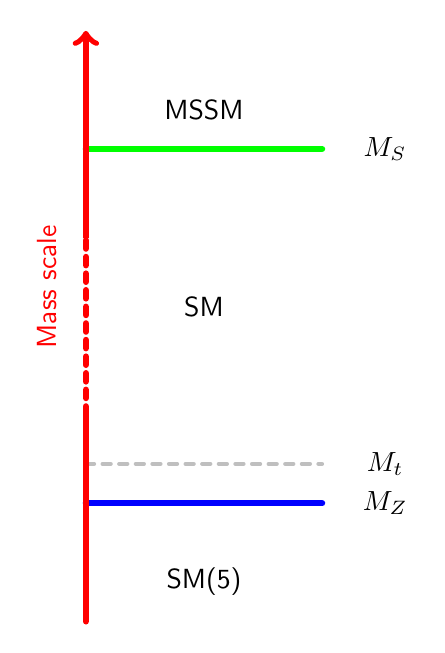
\begin{tikzpicture}
    % MSSM
    \node at (1.5,6) {\textsf{MSSM}};
    \draw[line width=0.08cm, line cap=round, color=green] (0,5.5) -- (3,5.5);
    \node at (3.8,5.5) {$M_S$};
    % SM
    \node at (1.5,3.5) {\textsf{SM}};
    \draw[line width=0.08cm, line cap=round, color=blue] (0,1) -- (3,1);
    \draw[line width=0.05cm, dashed, line cap=round, color=lightgray] (0,1.5) -- (3,1.5);
    \node at (3.8,1.5) {$M_t$};
    \node at (1.5,0) {\textsf{SM(5)}};
    % Energy ax
    \draw[line width=0.08cm, line cap=round, color=red] (0,-0.5) -- (0,2.125);
    \draw[line width=0.08cm, line cap=round, dashed, color=red] (0,2.125) -- (0,4.375);
    \draw[->, line width=0.08cm, color=red] (0,4.375) -- (0,7);
    % Ax label
    \node[rotate=90, color=red] at (-0.5,3.75) {\textsf{Mass scale}};
    % Threshold/scale labels
    \node at (3.8,1) {$M_Z$};
  \end{tikzpicture}}\hfill
  \resizebox{0.3\textwidth}{!}{%
  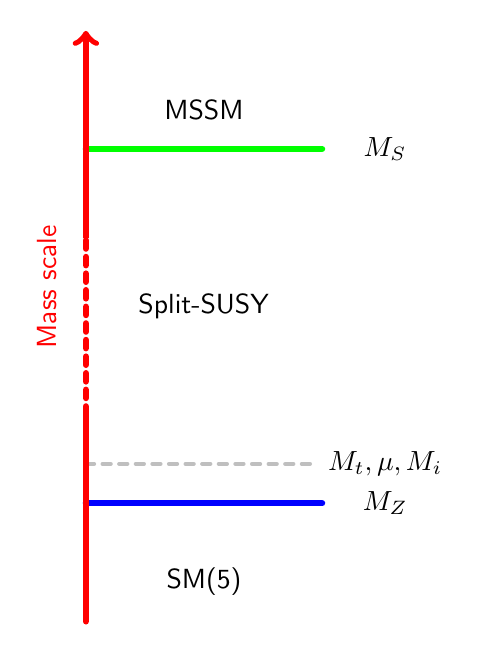
\begin{tikzpicture}
    % MSSM
    \node at (1.5,6) {\textsf{MSSM}};
    \draw[line width=0.08cm, line cap=round, color=green] (0,5.5) -- (3,5.5);
    \node at (3.8,5.5) {$M_S$};
    % Split SUSY
    \node at (1.5,3.5) {\textsf{Split-SUSY}};
    \draw[line width=0.08cm, line cap=round, color=blue] (0,1) -- (3,1);
    \draw[line width=0.05cm, dashed, line cap=round, color=lightgray] (0,1.5) -- (2.9,1.5);
    \node at (3.8,1.5) {$M_t, \mu, M_i$};
    \node at (1.5,0) {\textsf{SM(5)}};
    % Energy ax
    \draw[line width=0.08cm, line cap=round, color=red] (0,-0.5) -- (0,2.125);
    \draw[line width=0.08cm, line cap=round, dashed, color=red] (0,2.125) -- (0,4.375);
    \draw[->, line width=0.08cm, color=red] (0,4.375) -- (0,7);
    % Ax label
    \node[rotate=90, color=red] at (-0.5,3.75) {\textsf{Mass scale}};
    % Threshold/scale labels
    \node at (3.8,1) {$M_Z$};
  \end{tikzpicture}}\hfill
  \resizebox{0.3\textwidth}{!}{%
  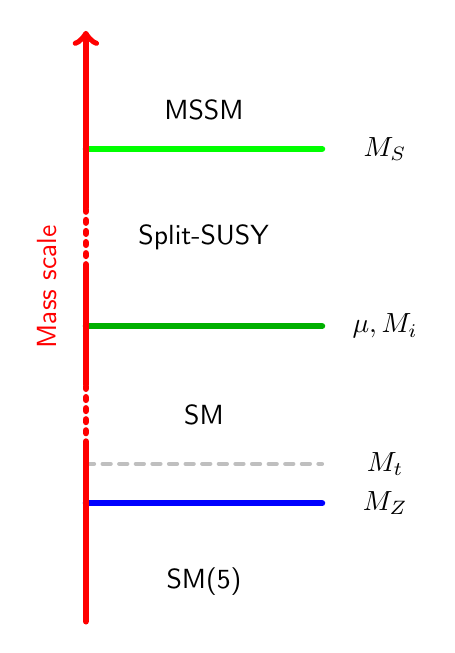
\begin{tikzpicture}
    % MSSM
    \node at (1.5,6) {\textsf{MSSM}};
    \draw[line width=0.08cm, line cap=round, color=green] (0,5.5) -- (3,5.5);
    \node at (3.8,5.5) {$M_S$};
    % Split SUSY
    \node at (1.5,4.375) {\textsf{Split-SUSY}};
    \draw[line width=0.08cm, line cap=round, color=darkgreen] (0,3.250) -- (3,3.250);
    \node at (3.8,3.250) {$\mu, M_i$};
    % SM
    \node at (1.5,2.125) {\textsf{SM}};
    \draw[line width=0.08cm, line cap=round, color=blue] (0,1) -- (3,1);
    \draw[line width=0.05cm, line cap=round, dashed, color=lightgray] (0,1.5) -- (3.,1.5);
    \node at (3.8,1.5) {$M_t$};
    \node at (1.5,0) {\textsf{SM(5)}};
    \node at (3.8,1) {$M_Z$};
    % Energy ax
    \draw[line width=0.08cm, line cap=round, color=red] (0,-0.5) -- (0,1.75);
    \draw[line width=0.08cm, line cap=round, dash pattern=on 1pt off 3pt, color=red] (0,1.75) -- (0,2.50);
    \draw[line width=0.08cm, color=red] (0,2.50) -- (0,4);
    \draw[line width=0.08cm, line cap=round, dash pattern=on 1pt off 3pt, color=red] (0,4) -- (0,4.75);
    \draw[->, line width=0.08cm, color=red] (0,4.75) -- (0,7);
    % Ax label
    \node[rotate=90, color=red] at (-0.5,3.75) {\textsf{Mass scale}};
  \end{tikzpicture}}
\end{frame}

\begin{frame}{EFT towers with low-scale 2HDM}
  \resizebox{0.3\textwidth}{!}{%
  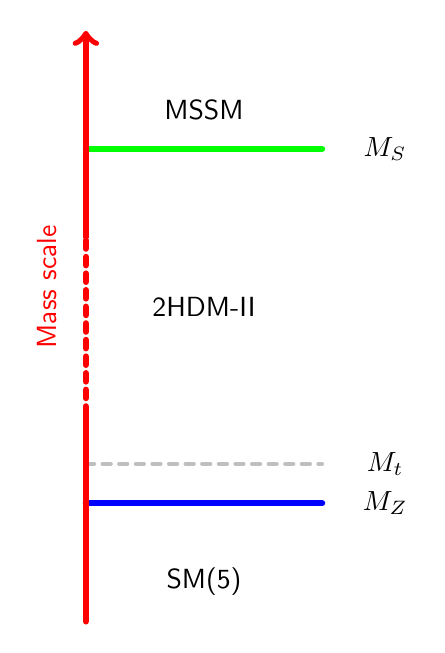
\begin{tikzpicture}
    % MSSM
    \node at (1.5,6) {\textsf{MSSM}};
    \draw[line width=0.08cm, line cap=round, color=green] (0,5.5) -- (3,5.5);
    \node at (3.8,5.5) {$M_S$};
    % SM
    \node at (1.5,3.5) {\textsf{2HDM-II}};
    \draw[line width=0.08cm, line cap=round, color=blue] (0,1) -- (3,1);
    \draw[line width=0.05cm, dashed, line cap=round, color=lightgray] (0,1.5) -- (3,1.5);
    \node at (3.8,1.5) {$M_t$};
    \node at (1.5,0) {\textsf{SM(5)}};
    % Energy ax
    \draw[line width=0.08cm, line cap=round, color=red] (0,-0.5) -- (0,2.125);
    \draw[line width=0.08cm, line cap=round, dashed, color=red] (0,2.125) -- (0,4.375);
    \draw[->, line width=0.08cm, color=red] (0,4.375) -- (0,7);
    % Ax label
    \node[rotate=90, color=red] at (-0.5,3.75) {\textsf{Mass scale}};
    % Threshold/scale labels

    \node at (3.8,1) {$M_Z$};
  \end{tikzpicture}}\hfill
  \resizebox{0.3\textwidth}{!}{%
    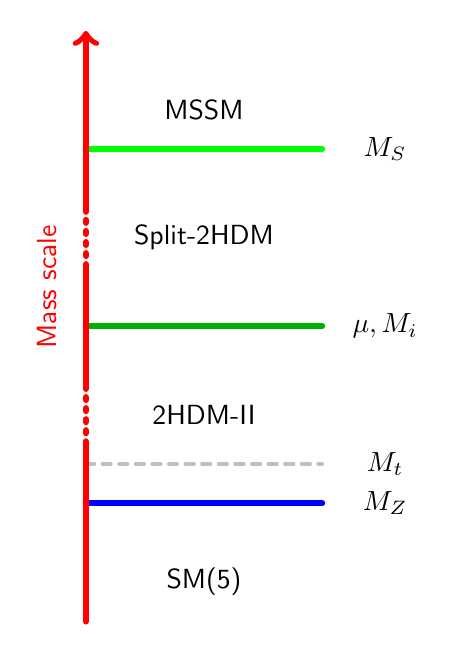
\begin{tikzpicture}
    % MSSM
    \node at (1.5,6) {\textsf{MSSM}};
    \draw[line width=0.08cm, line cap=round, color=green] (0,5.5) -- (3,5.5);
    \node at (3.8,5.5) {$M_S$};
    % Split SUSY
    \node at (1.5,4.375) {\textsf{Split-2HDM}};
    \draw[line width=0.08cm, line cap=round, color=darkgreen] (0,3.250) -- (3,3.250);
    \node at (3.8,3.250) {$\mu, M_i$};
    % SM
    \node at (1.5,2.125) {\textsf{2HDM-II}};
    \draw[line width=0.08cm, line cap=round, color=blue] (0,1) -- (3,1);
    \draw[line width=0.05cm, line cap=round, dashed, color=lightgray] (0,1.5) -- (3.,1.5);
    \node at (3.8,1.5) {$M_t$};
    \node at (1.5,0) {\textsf{SM(5)}};
    \node at (3.8,1) {$M_Z$};
    % Energy ax
    \draw[line width=0.08cm, line cap=round, color=red] (0,-0.5) -- (0,1.75);
    \draw[line width=0.08cm, line cap=round, dash pattern=on 1pt off 3pt, color=red] (0,1.75) -- (0,2.50);
    \draw[line width=0.08cm, color=red] (0,2.50) -- (0,4);
    \draw[line width=0.08cm, line cap=round, dash pattern=on 1pt off 3pt, color=red] (0,4) -- (0,4.75);
    \draw[->, line width=0.08cm, color=red] (0,4.75) -- (0,7);
    % Ax label
    \node[rotate=90, color=red] at (-0.5,3.75) {\textsf{Mass scale}};
  \end{tikzpicture}}\hfill
  \resizebox{0.3\textwidth}{!}{%
   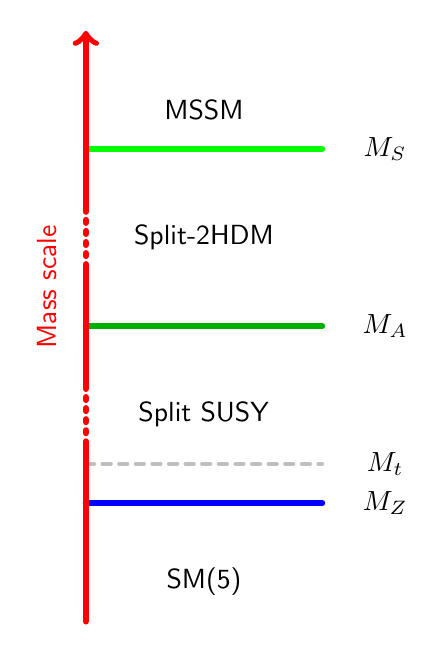
\begin{tikzpicture}
    % MSSM
    \node at (1.5,6) {\textsf{MSSM}};
    \draw[line width=0.08cm, line cap=round, color=green] (0,5.5) -- (3,5.5);
    \node at (3.8,5.5) {$M_S$};
    % Split SUSY
    \node at (1.5,4.375) {\textsf{Split-2HDM}};
    \draw[line width=0.08cm, line cap=round, color=darkgreen] (0,3.250) -- (3,3.250);
    \node at (3.8,3.250) {$M_A$};
    % SM
    \node at (1.5,2.125) {\textsf{Split SUSY}};
    \draw[line width=0.08cm, line cap=round, color=blue] (0,1) -- (3,1);
    \draw[line width=0.05cm, line cap=round, dashed, color=lightgray] (0,1.5) -- (3.,1.5);
    \node at (3.8,1.5) {$M_t$};
    \node at (1.5,0) {\textsf{SM(5)}};
    \node at (3.8,1) {$M_Z$};
    % Energy ax
    \draw[line width=0.08cm, line cap=round, color=red] (0,-0.5) -- (0,1.75);
    \draw[line width=0.08cm, line cap=round, dash pattern=on 1pt off 3pt, color=red] (0,1.75) -- (0,2.50);
    \draw[line width=0.08cm, color=red] (0,2.50) -- (0,4);
    \draw[line width=0.08cm, line cap=round, dash pattern=on 1pt off 3pt, color=red] (0,4) -- (0,4.75);
    \draw[->, line width=0.08cm, color=red] (0,4.75) -- (0,7);
    % Ax label
    \node[rotate=90, color=red] at (-0.5,3.75) {\textsf{Mass scale}};
  \end{tikzpicture}}
\end{frame}

%%%%%%%%%%%%%%%%%%%%%%%%%%%%%%%%%%%%%%%%

\section{Automatic uncertainty estimates}

\begin{frame}{$M_h$ in the MSSM at fixed loop order}
  Large cancellations:\\
  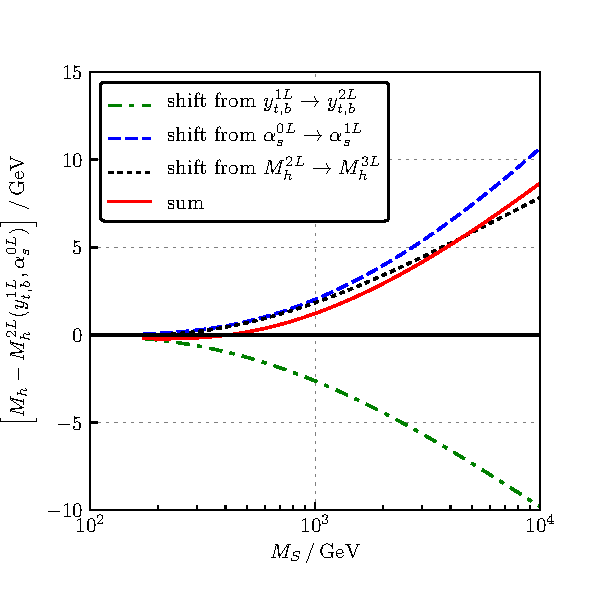
\includegraphics[width=0.49\textwidth]{plots/Mh3L/scan_Mh_MS_TB-5_Xt-0_contributions}\hfill
  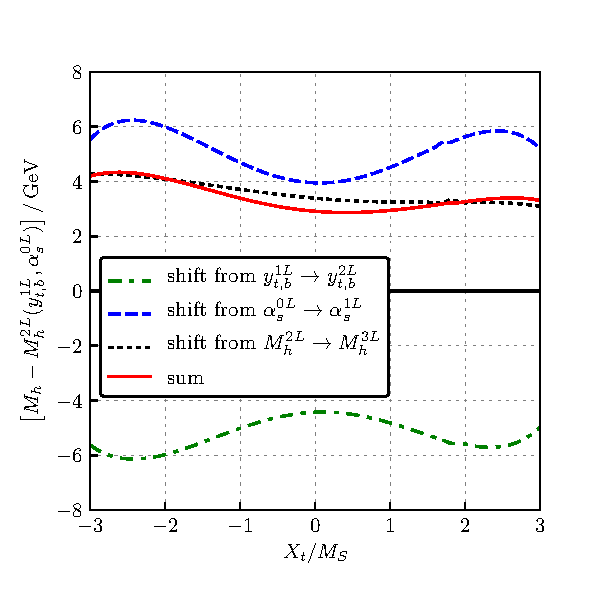
\includegraphics[width=0.49\textwidth]{plots/Mh3L/scan_Mh_Xt_TB-5_MS-2000_contributions}\\
  $\tan\beta=5$, $X_t=0$, $\MS = 2\eh{TeV}$
\end{frame}

\begin{frame}{$M_h$ in the MSSM at fixed loop order}
  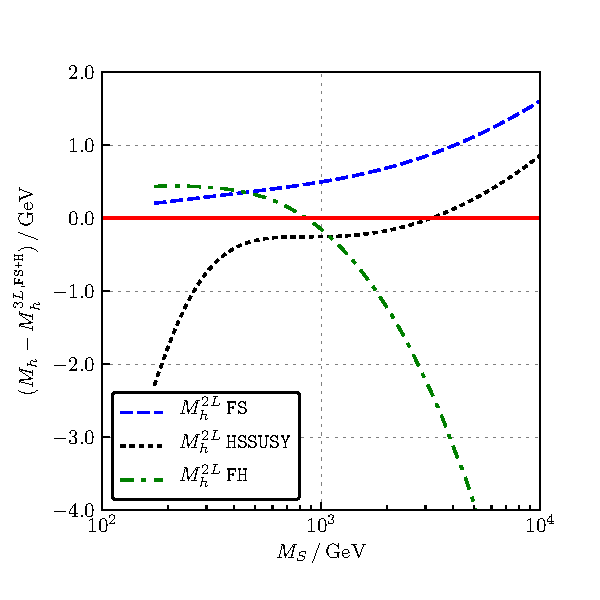
\includegraphics[width=0.49\textwidth]{plots/Mh3L/scan_Mh_MS_TB-5_Xt-0_diff}\hfill
  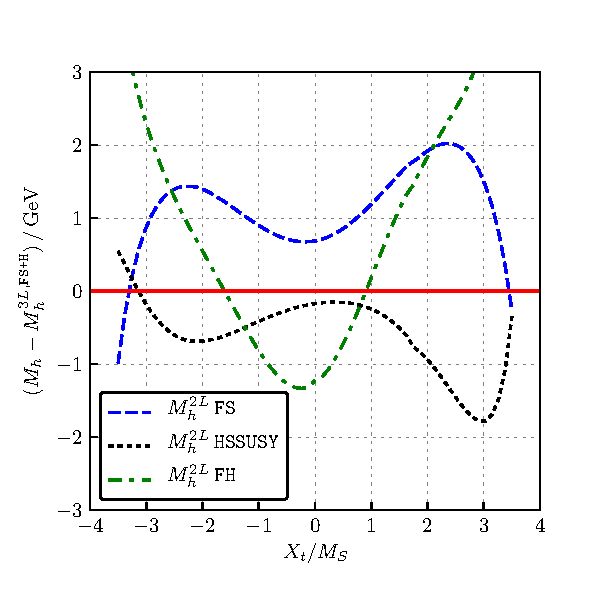
\includegraphics[width=0.49\textwidth]{plots/Mh3L/scan_Mh_Xt_TB-5_MS-2000_diff}\\
  $\tan\beta=5$, $X_t=0$, $\MS = 2\eh{TeV}$
\end{frame}

\begin{frame}{Requirements for uncertainty estimate}
  \begin{itemize}
  \item code specific
  \item flag specific
  \item generic (MSSM, NMSSM, THDM, \ldots)
  \item $\MS \lesssim 1\eh{TeV}$: envelope fixed order 3-loop calculation
  \item $\MS \gtrsim 1\eh{TeV}$: envelope EFT 2-loop calculation
  \end{itemize}
\end{frame}

\begin{frame}{Debatable ways to calculate $\Delta M_h$}
  \begin{center}
  \begin{tabular}{lllll}
    \toprule
    fixed order & 1L & 2L & 3L \\
    \midrule
    $Q_\pole$ & $[\MS/2, 2\MS]$ & $[\MS/2, 2\MS]$ & $[\MS/2, 2\MS]$ \\
    $y_t(M_Z)$ & 0L vs.\ 1L & 1L vs.\ 2L & \textcolor{red}{2L vs.\ 3L} \\
    $\alpha_s(M_Z)$ & 0L vs.\ 1L & 1L vs.\ 2L & \textcolor{red}{2L vs.\ 3L} \\
    \midrule
    EFT/mixed & $\Delta\lambda^{0L}$ & $\Delta\lambda^{1L}$ & $\Delta\lambda^{2L}$ \\
    \midrule
    $Q_\text{match}$ & $[\MS/2, 2\MS]$ & $[\MS/2, 2\MS]$ & $[\MS/2, 2\MS]$ \\
    $\lambda(\MS)$ & $0$ vs.\ $\frac{v^2}{\MS^2}$ & $0$ vs.\ $\frac{v^2}{\MS^2}$ & $0$ vs.\ $\frac{v^2}{\MS^2}$ \\
    \midrule
    EFT/mixed & $\Delta M_h^{1L}$, $\beta^{1L}$ & $\Delta M_h^{2L}$, $\beta^{2L}$ & $\Delta M_h^{3L}$, $\beta^{3L}$ \\
    \midrule
    $Q_\pole$ & $[M_t/2, 2M_t]$ & $[M_t/2, 2M_t]$ & $[M_t/2, 2M_t]$ \\
    $y_t(M_Z)$ & 0L vs.\ 1L & 1L vs.\ 2L & 2L vs.\ 3L \\
    $\alpha_s(M_Z)$ & 0L vs.\ 1L & 1L vs.\ 2L & 2L vs.\ 3L \\
    \bottomrule
  \end{tabular}
\end{center}
\end{frame}

%%%%%%%%%%%%%%%%%%%%%%%%%%%%%%%%%%%%%%%%
% backup slides
%%%%%%%%%%%%%%%%%%%%%%%%%%%%%%%%%%%%%%%%

\begin{frame}[noframenumbering]
  \begin{center}
    \Huge Backup
  \end{center}
\end{frame}

\end{document}
